\begin{figure}
    \centering
    \begin{subfigure}{0.235\textwidth}
        \centering
        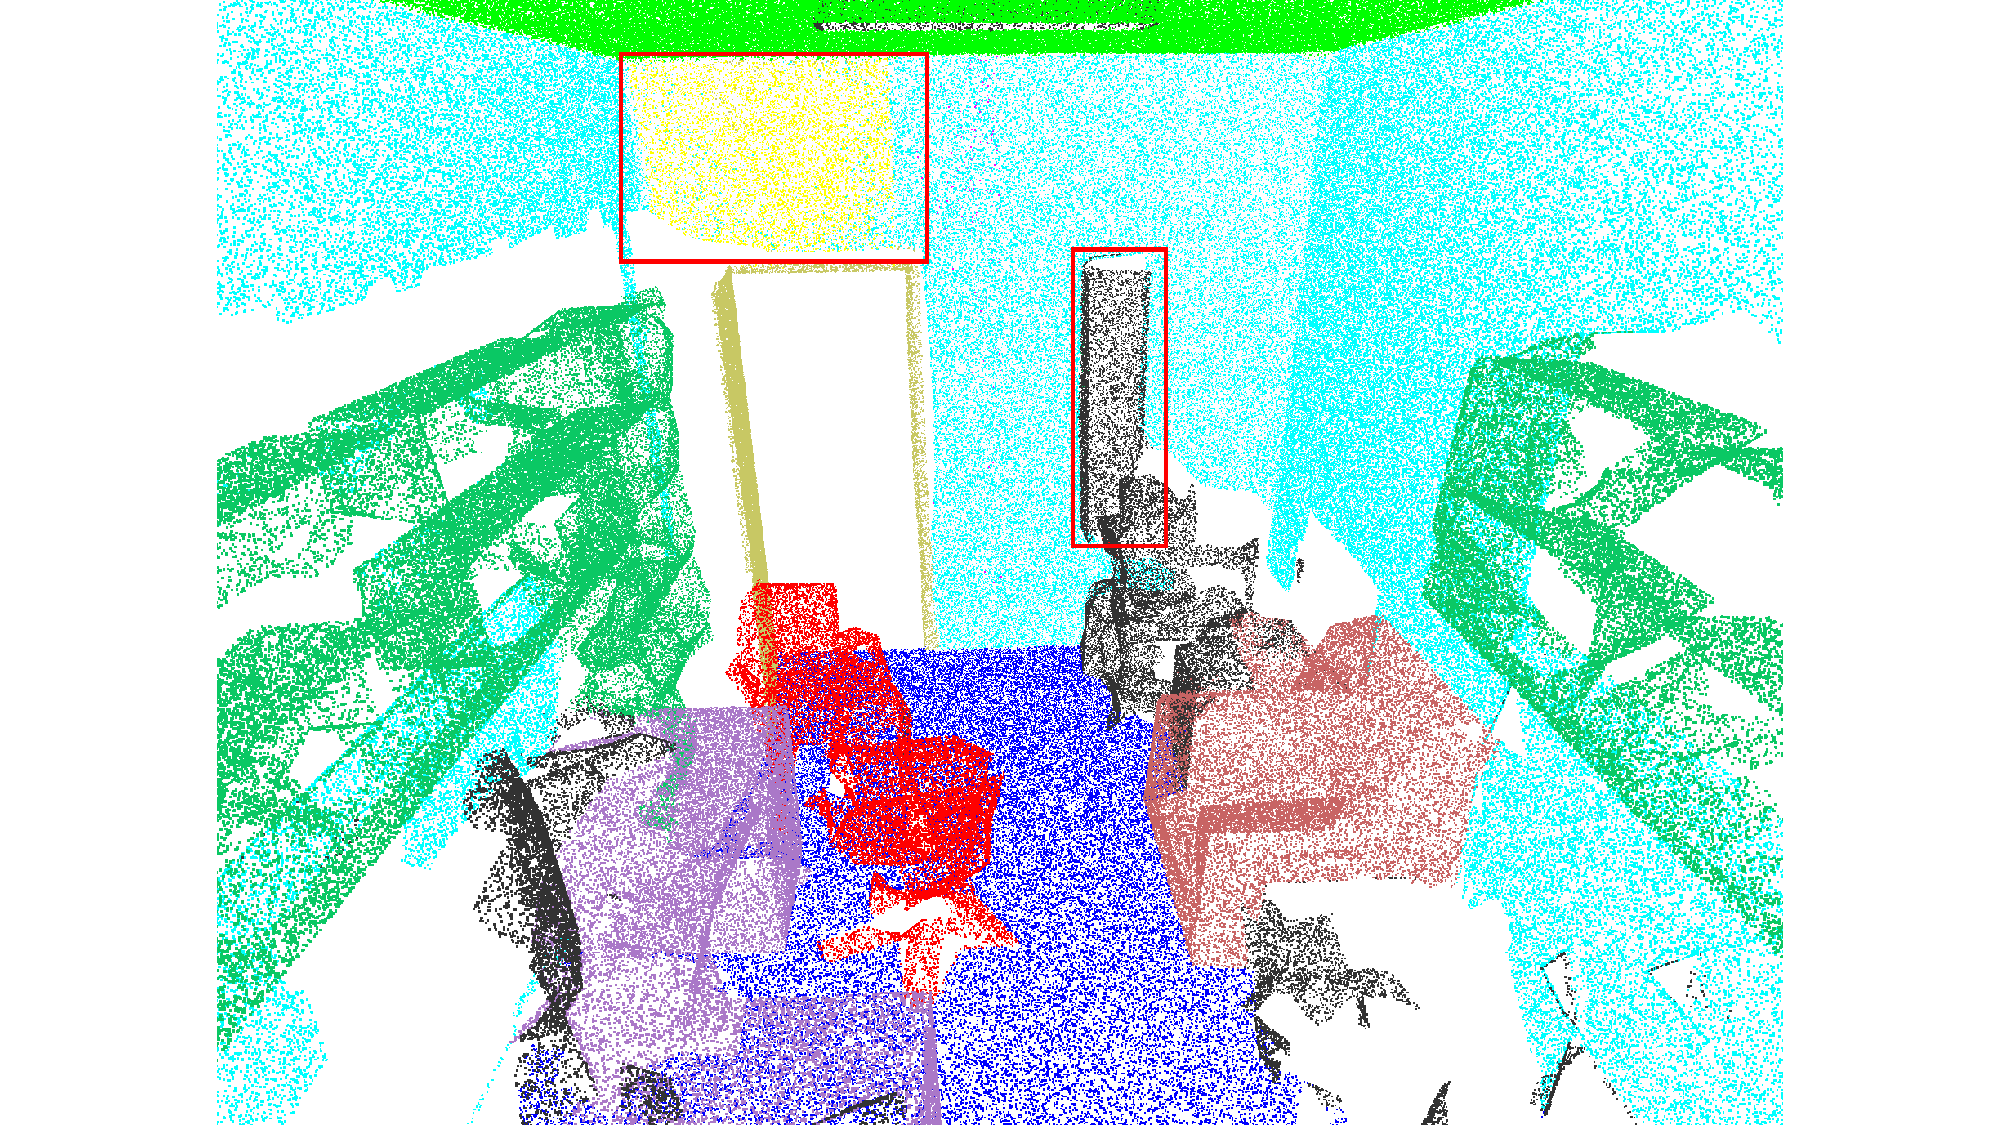
\includegraphics[width=\linewidth]{fig/S3DIS/PointMAE.pdf}
        % \caption*{\textbf{\#TP}:22.1M \textbf{\#OA}:85.18}
        \caption{Full fine-tuning}
        \label{fig:s3dis1}
    \end{subfigure}
    \hfill
    \begin{subfigure}{0.235\textwidth}
        \centering
        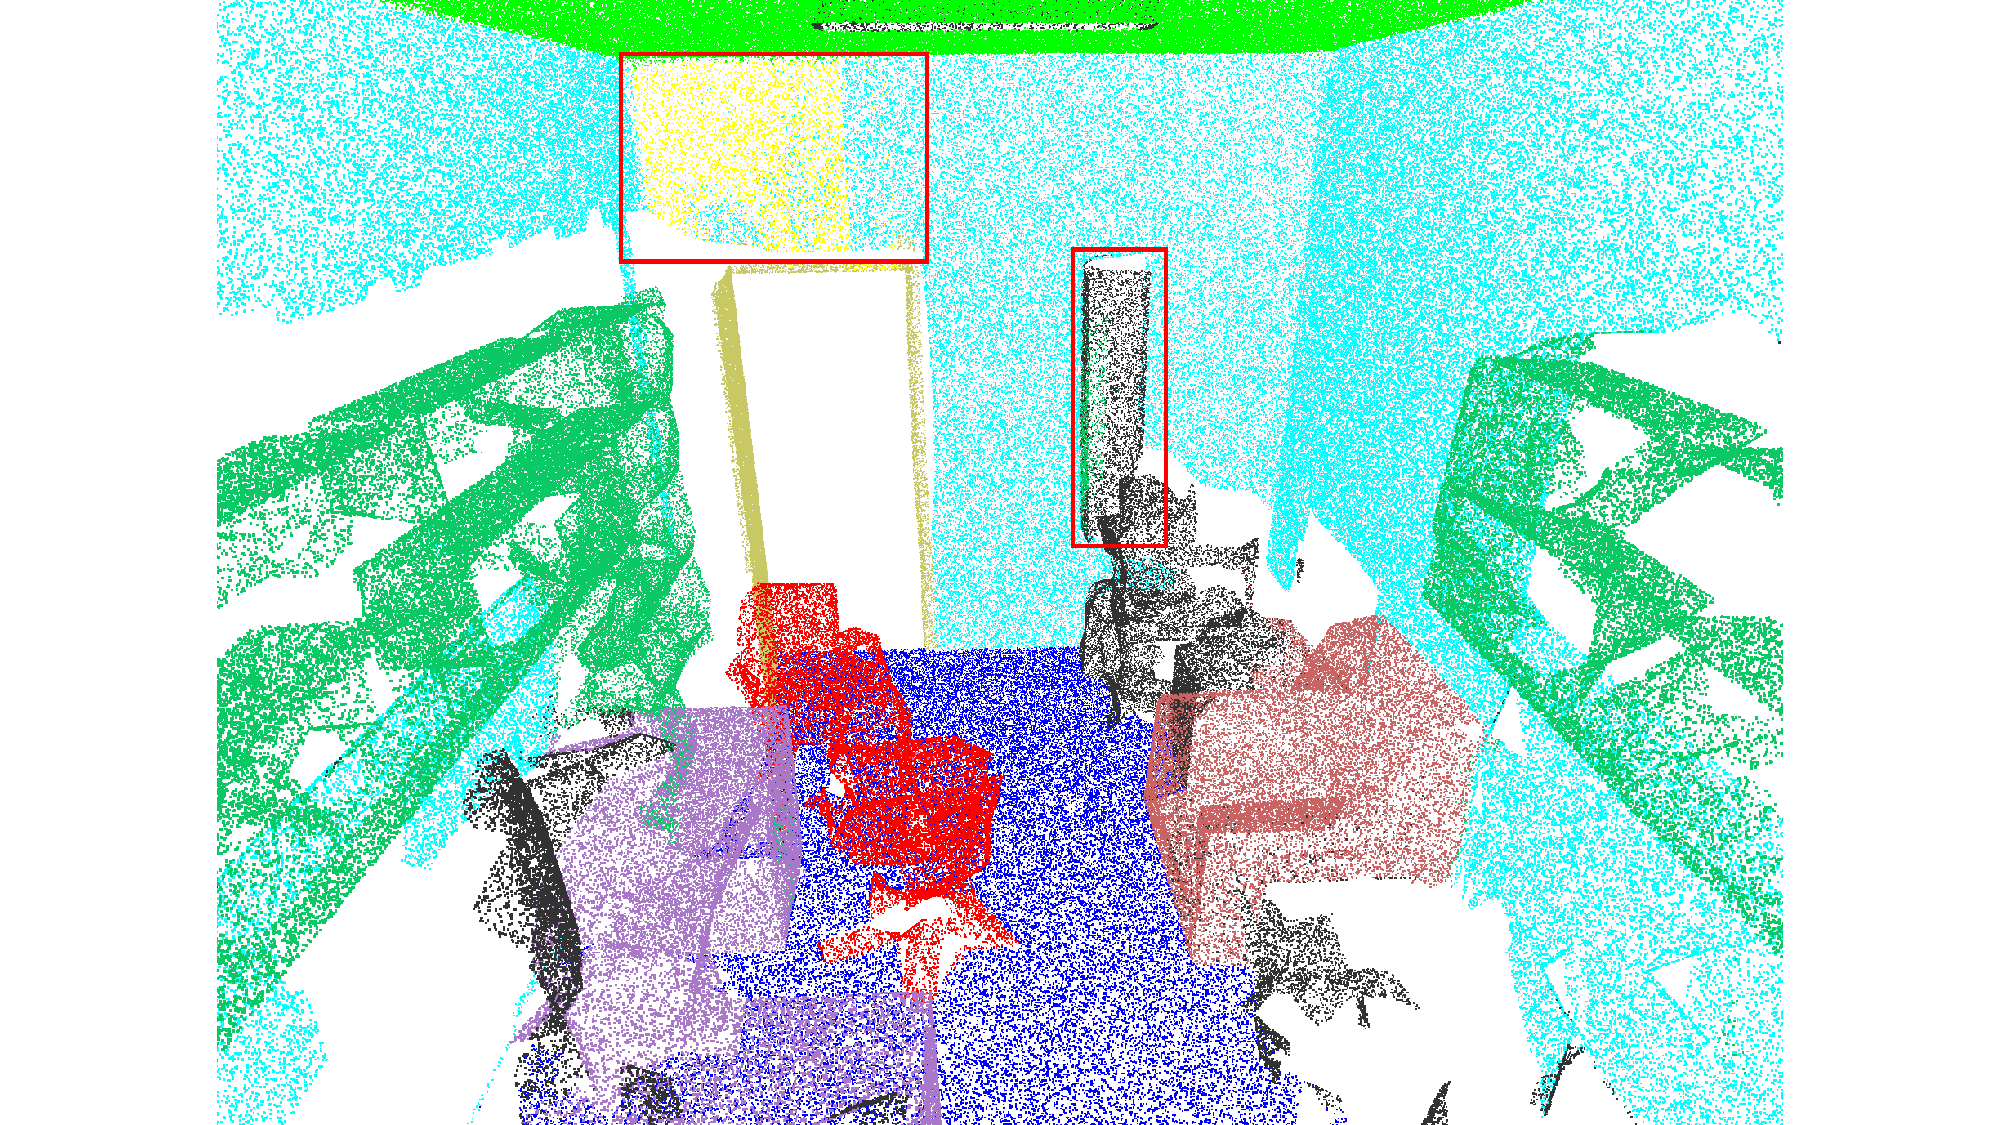
\includegraphics[width=\linewidth]{fig/S3DIS/DAPT.pdf}
        % \caption*{\textbf{\#TP}:1.7M \textbf{\#OA}:84.94}
        \caption{DAPT~\cite{zhou2024dynamic}}
        \label{fig:s3dis2}
    \end{subfigure}
    \hfill
    \begin{subfigure}{0.235\textwidth}
        \centering
        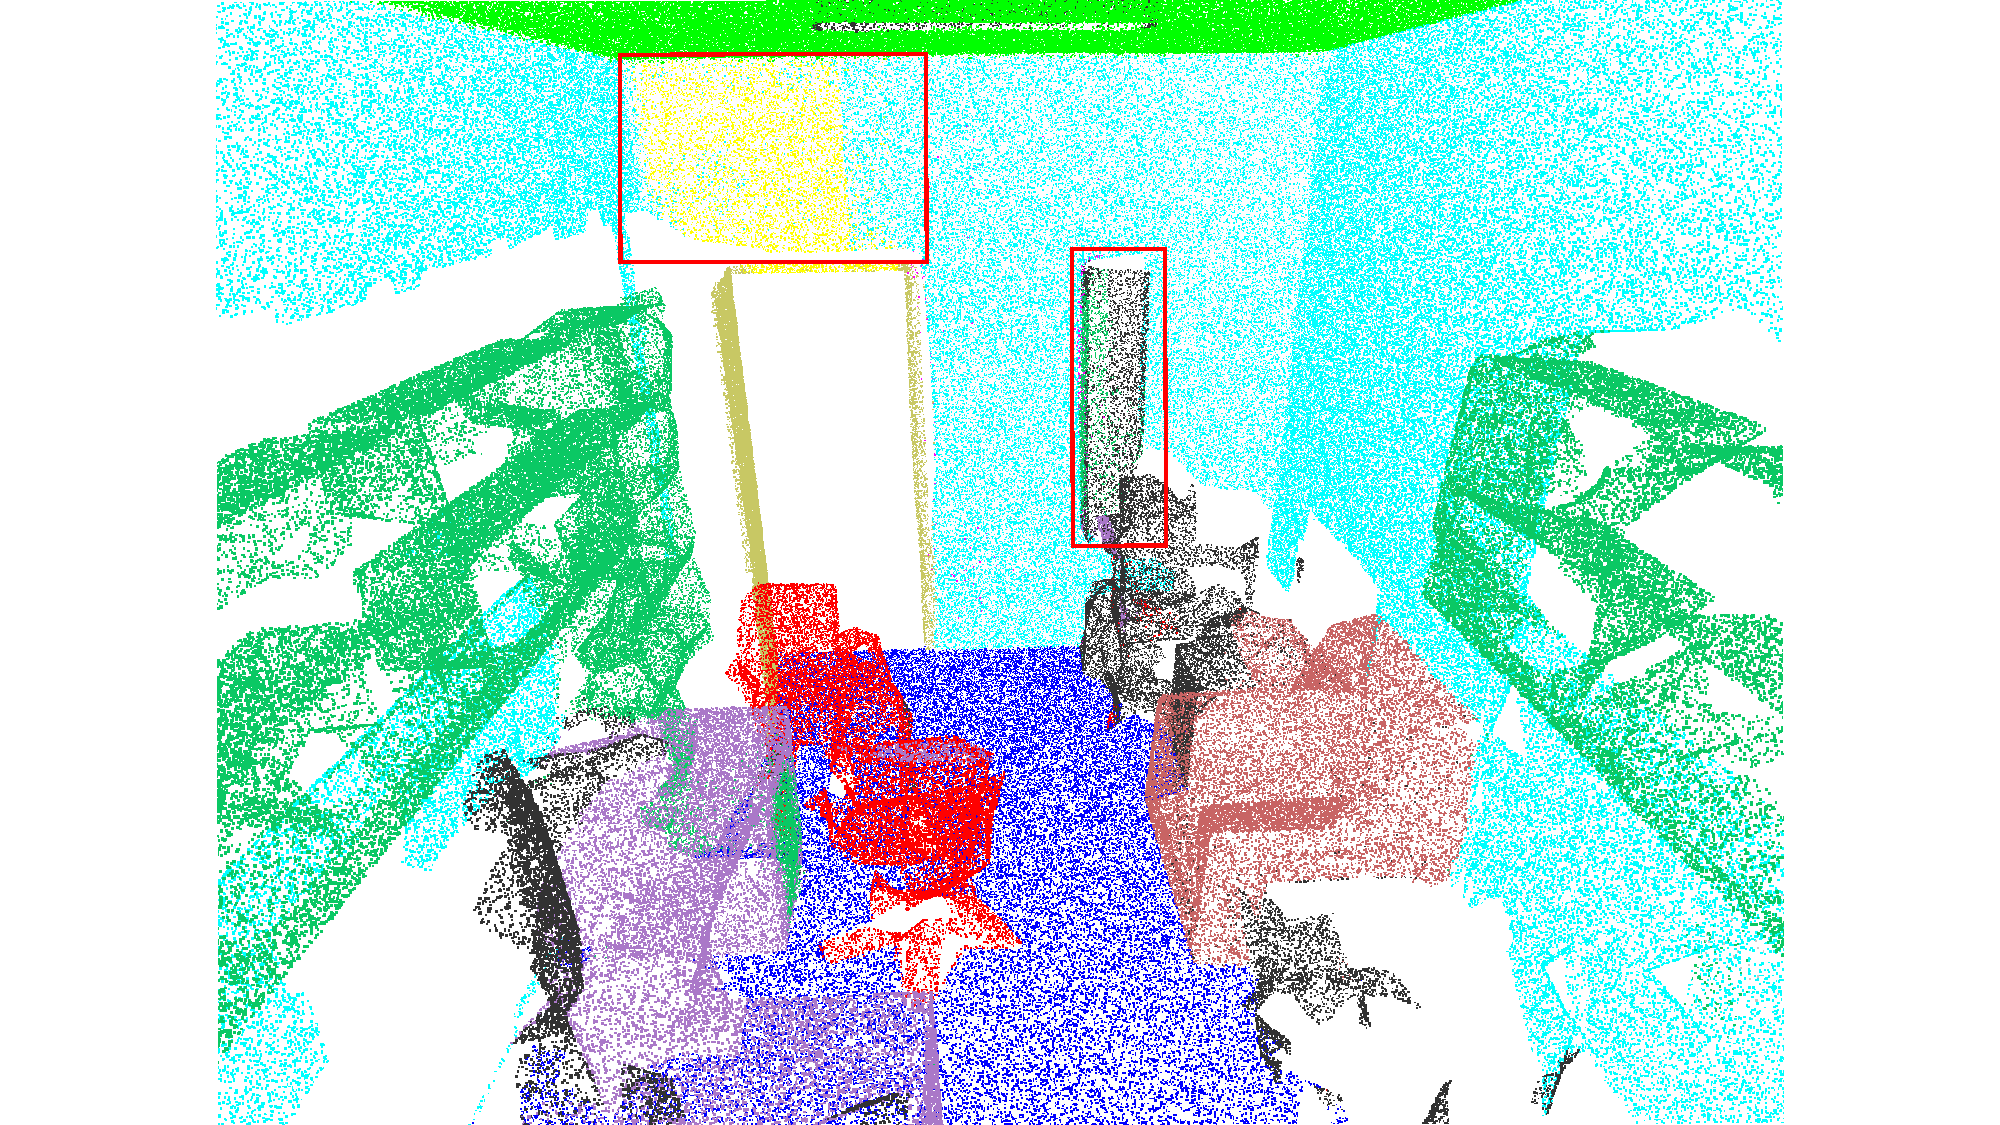
\includegraphics[width=\linewidth]{fig/S3DIS/IDPT.pdf}
        % \caption*{\textbf{\#TP}:1.1M \textbf{\#OA}:85.08}
        \caption{IDPT~\cite{zha2023instance}}
        \label{fig:s3dis3}
    \end{subfigure}
    \hfill
    \begin{subfigure}{0.235\textwidth}
        \centering
        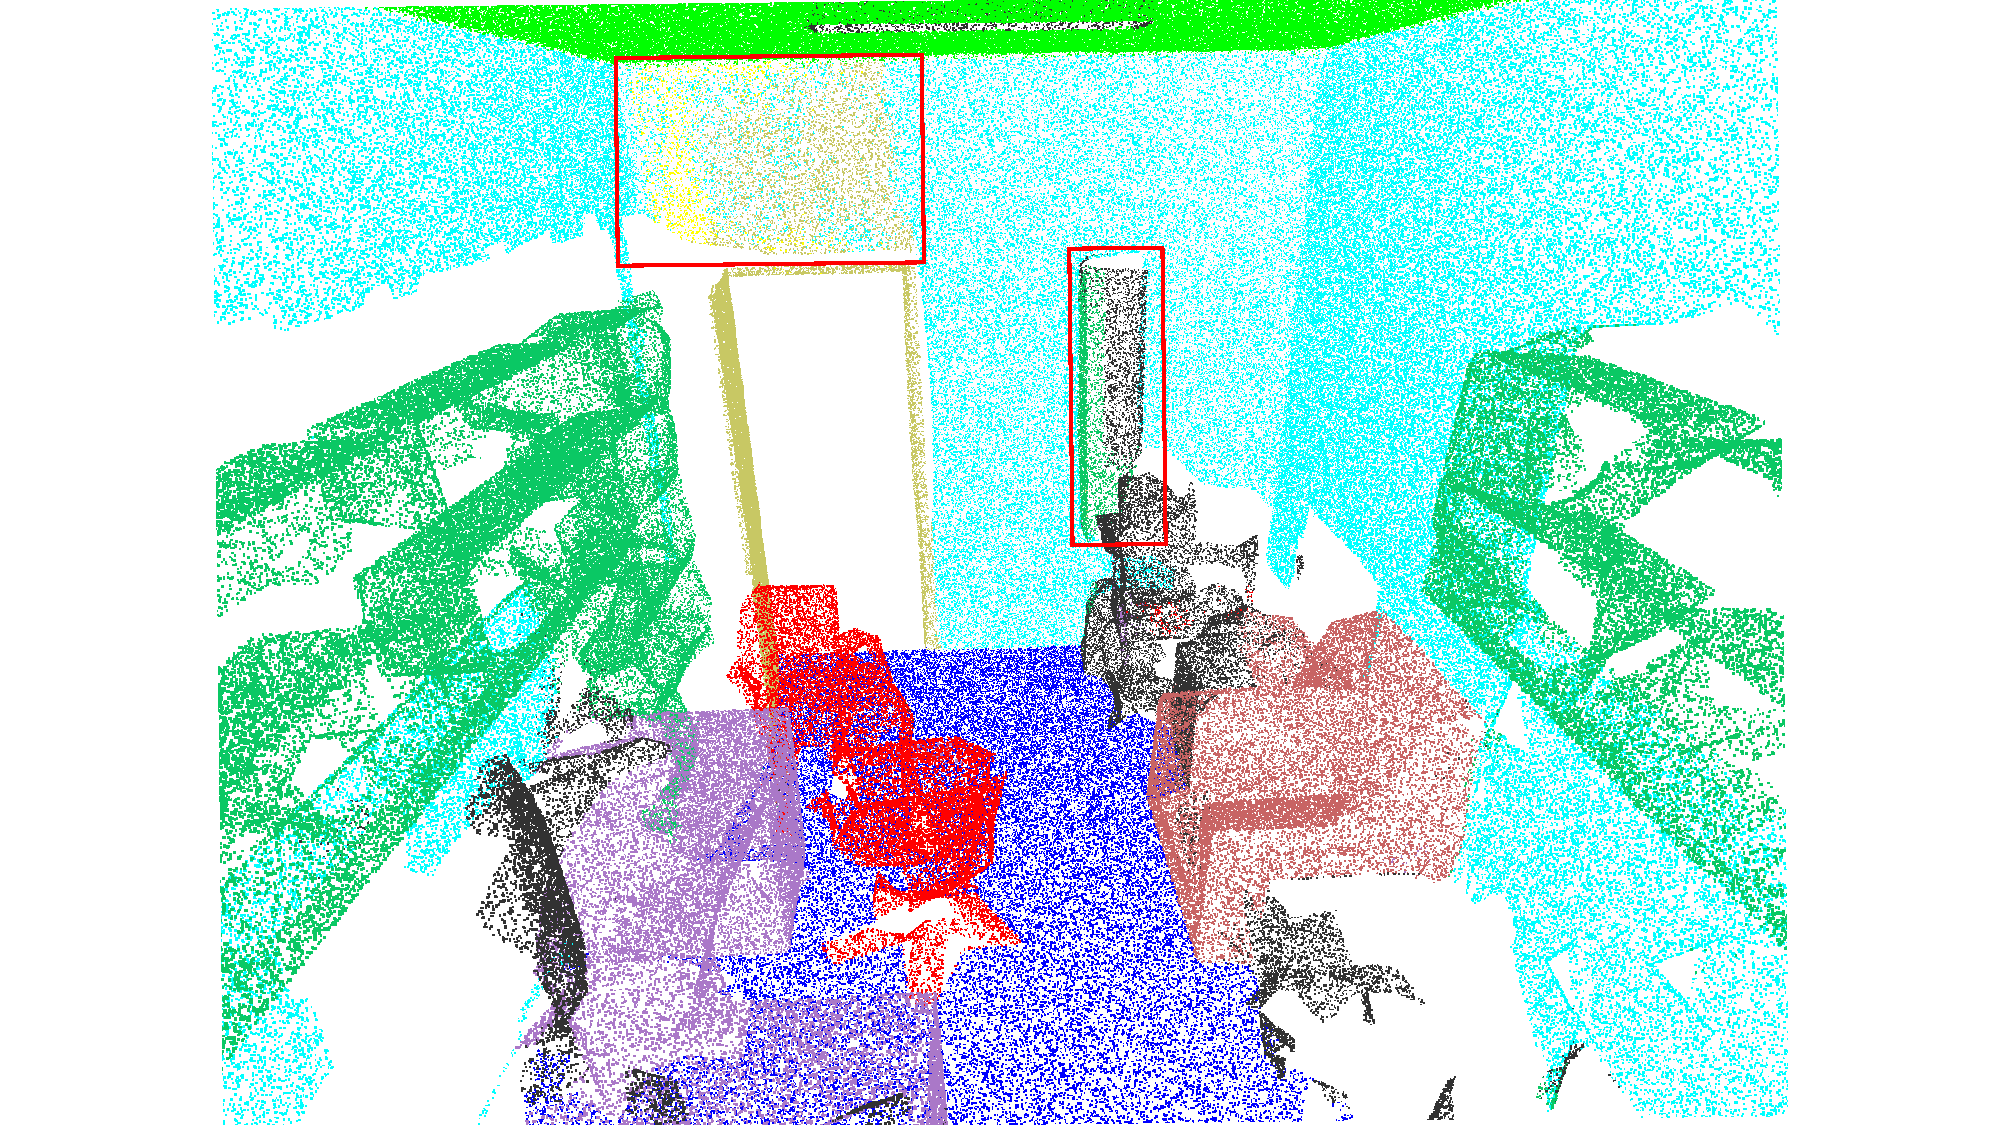
\includegraphics[width=\linewidth]{fig/S3DIS/PPT.pdf}
        % \caption*{\textbf{\#TP}:1.1M \textbf{\#OA}:84.91}
        \caption{PPT~\cite{zhang2024positional}}
        \label{fig:s3dis4}
    \end{subfigure}
    \hfill
    \begin{subfigure}{0.235\textwidth}
        \centering
        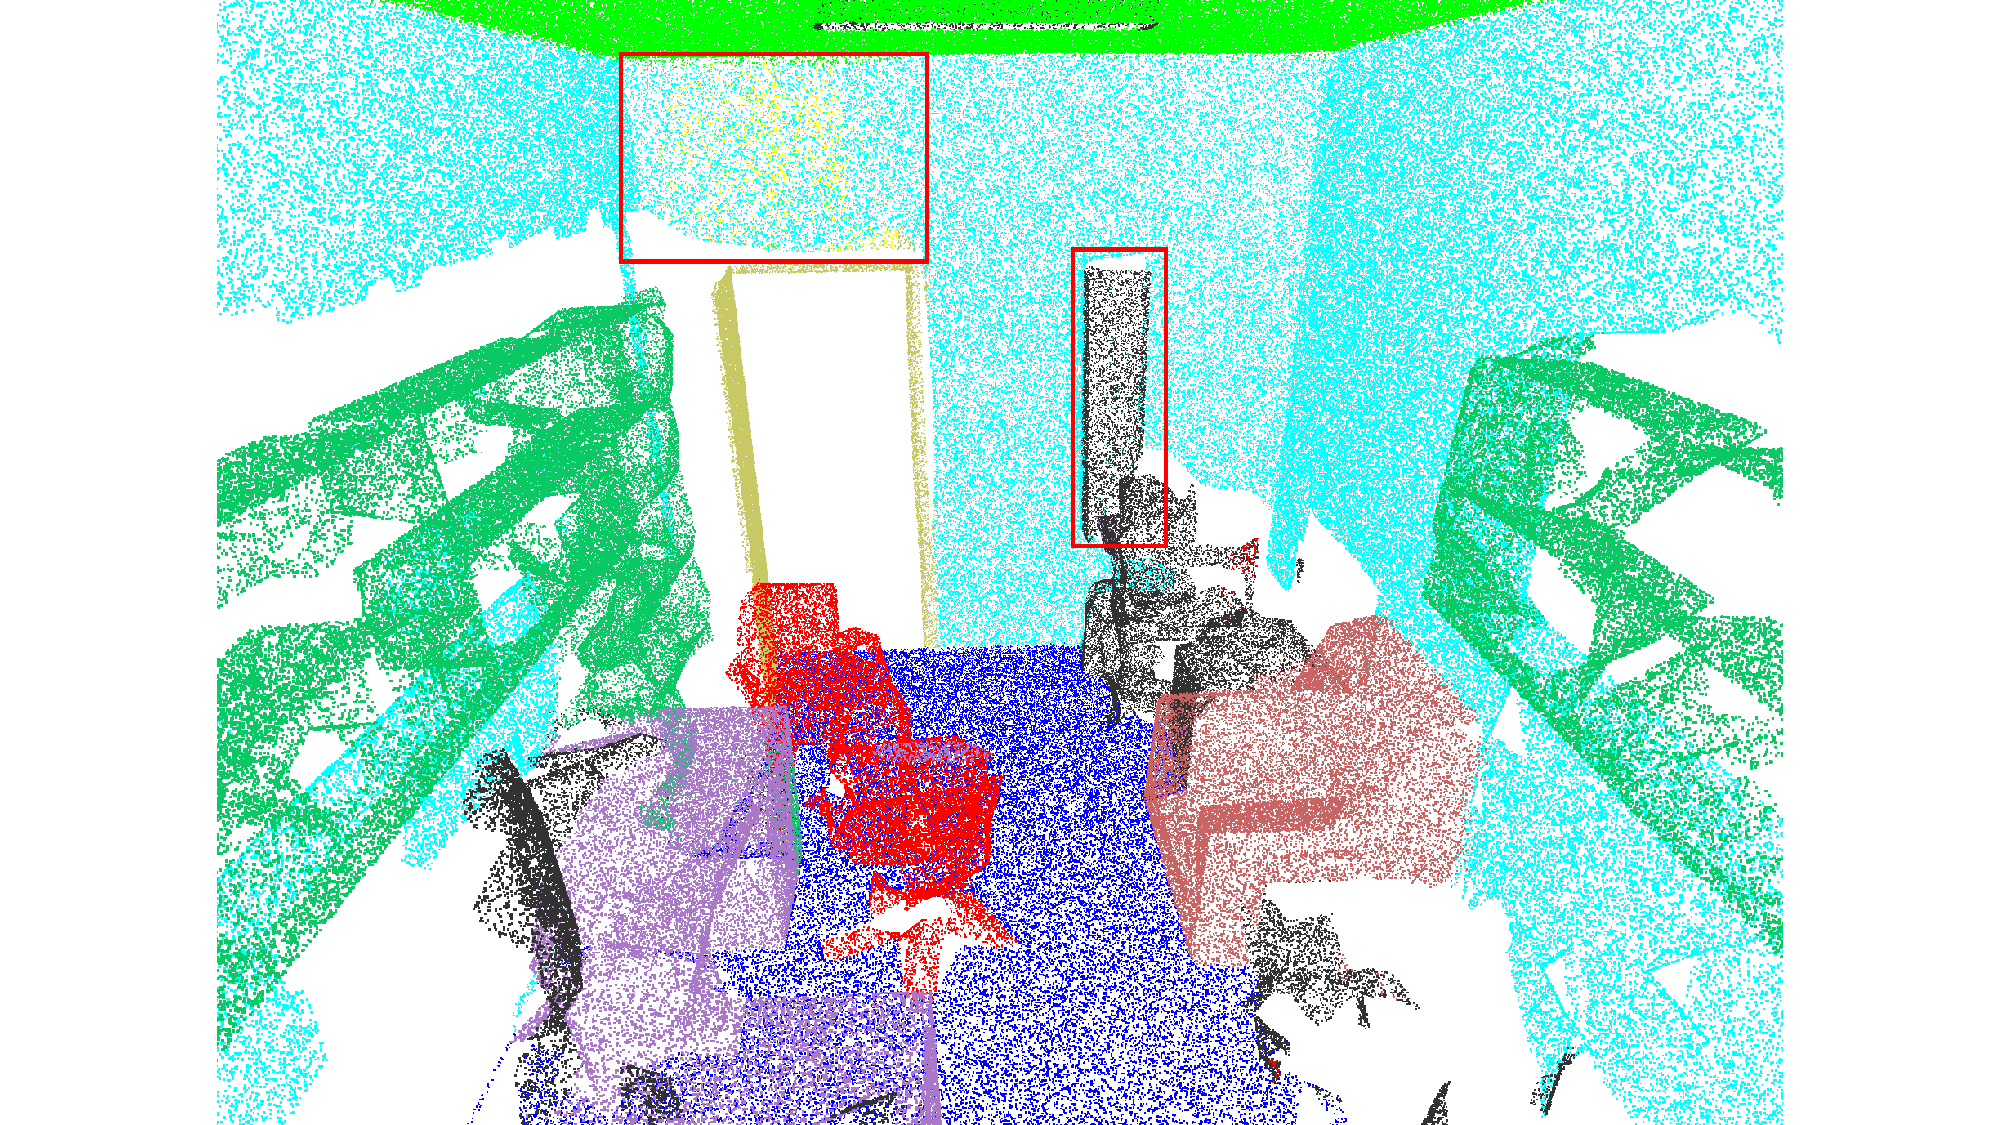
\includegraphics[width=\linewidth]{fig/S3DIS/PLT.pdf}
        % \caption*{\textbf{\#TP}:0.8M \textbf{\#OA}:82.75}
        \caption{PLT (Ours)}
        \label{fig:s3dis5}
    \end{subfigure}
    \hfill
    \begin{subfigure}{0.235\textwidth}
        \centering
        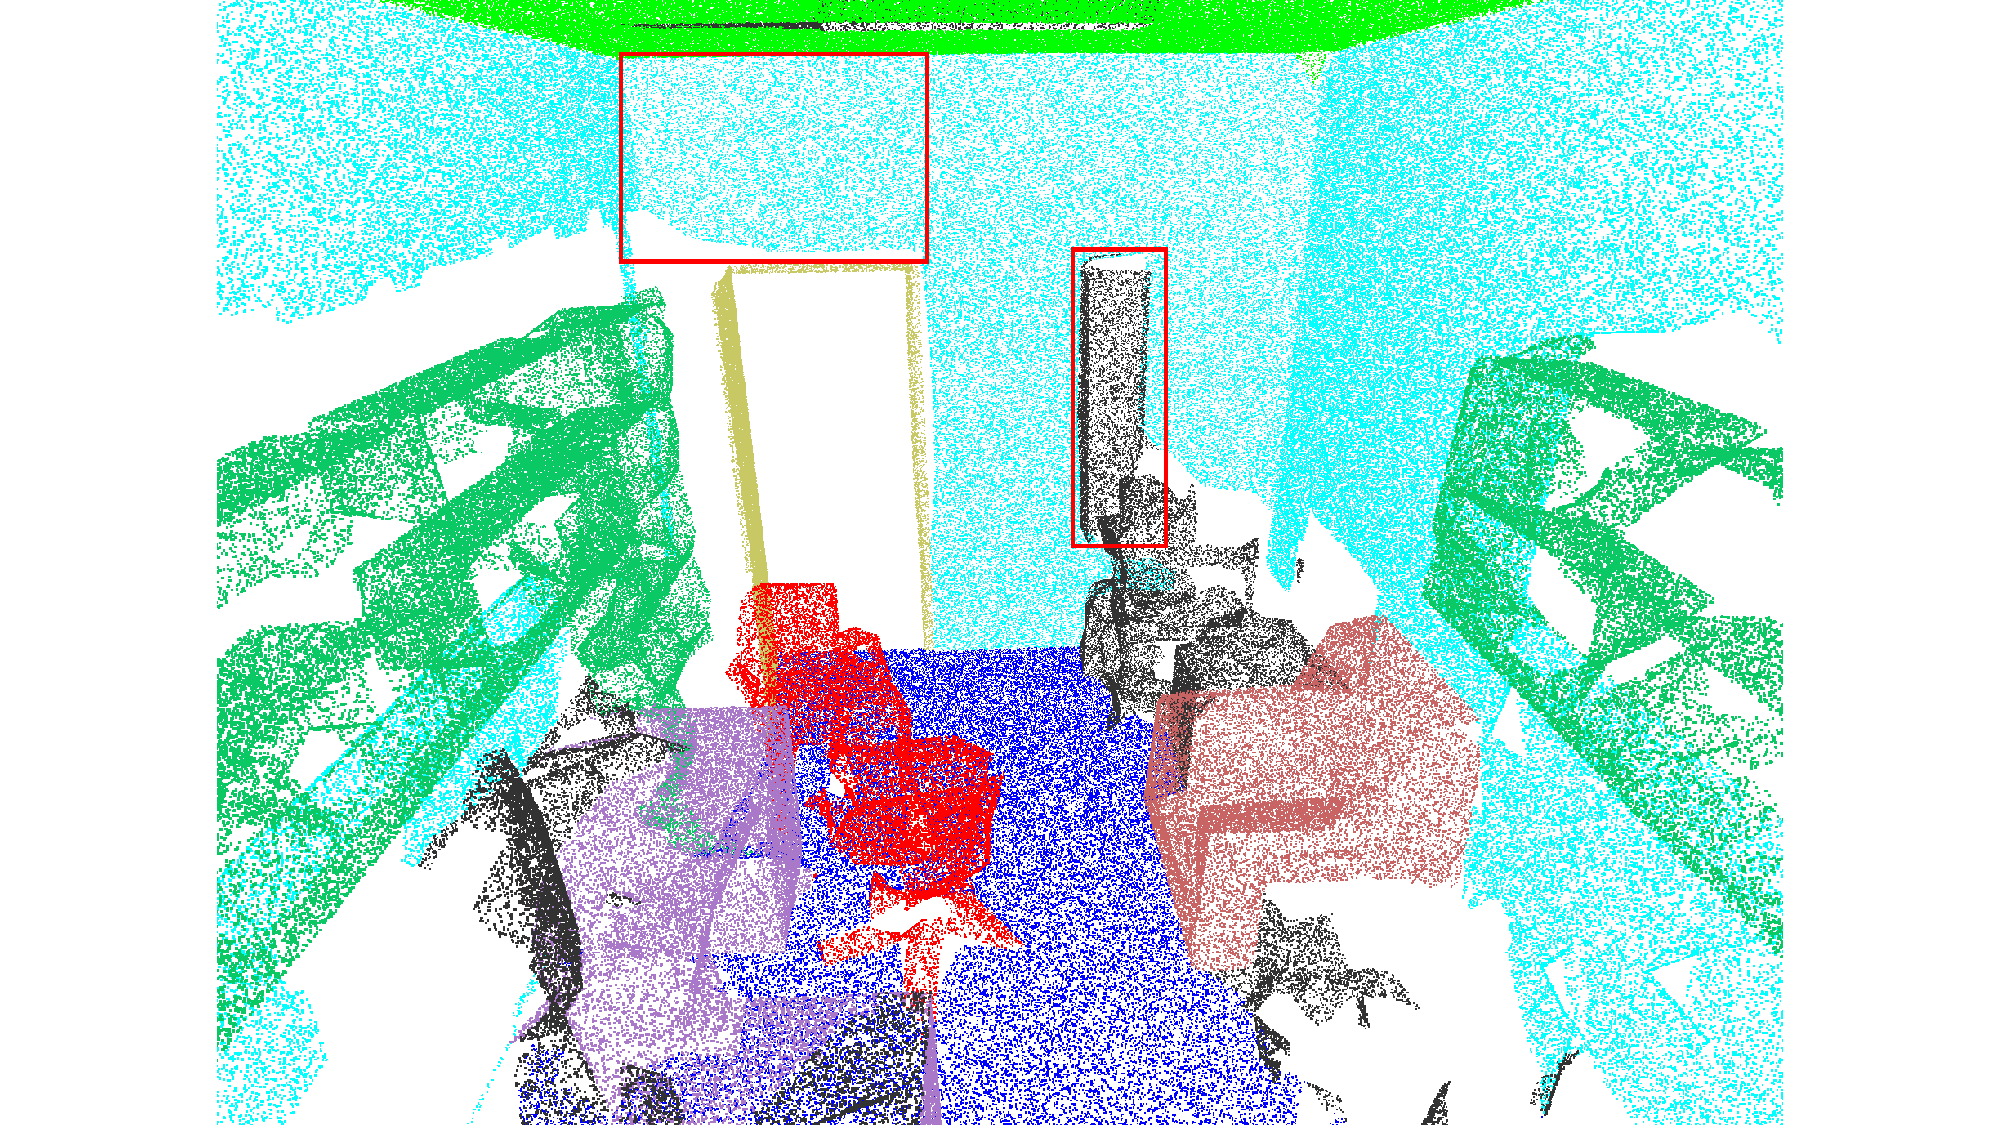
\includegraphics[width=\linewidth]{fig/S3DIS/GT.pdf}
        % \caption*{\textbf{\#TP}:0.6M \textbf{\#OA}:85.46}
        \caption{GT}
        \label{fig:s3dis6}
    \end{subfigure}
    \caption{The visualizations from the Area5 of S3DIS using a pre-trained PointMAE with various fine-tuning strategies.}
    \label{fig:s3dis}
\end{figure}